\documentclass[14pt, russian, a4paper]{extarticle}

% packages

\usepackage[a4paper, includefoot,
            left=2.5cm, right=1.5cm,
            top=1.5cm, bottom=1.5cm,
            headsep=1cm, footskip=1cm]{geometry}

\usepackage[utf8]{inputenc}
\usepackage[T2A]{fontenc}
\usepackage[english, main=russian]{babel}
\usepackage{graphicx}
\usepackage{amssymb}
\usepackage{amsfonts}
\usepackage{amsmath}
\usepackage{amsthm}
\usepackage{physics}
\usepackage{nicefrac}
\usepackage{cancel}
\usepackage{hyperref}
\usepackage{cmap}
\usepackage{tempora}
\usepackage{indentfirst}
\usepackage{multirow}

\newcommand{\Section}[1]{\clearpage % put new chapters on a new page
\refstepcounter{section} % manually increment the chapter number
% manually add the chapter to the table of contents
\addcontentsline{toc}{section}{\protect\numberline{\thesection.}#1}
% and now format the header according to spec.
\begin{center}
\textbf{\protect{\thesection.}\ \ #1}
\end{center}
}

\newcommand{\Subsection}[1]{% put new chapters on a new page
\refstepcounter{subsection} % manually increment the chapter number
% manually add the chapter to the table of contents
\addcontentsline{toc}{subsection}{\protect\numberline{\thesubsection.}#1}
% and now format the header according to spec.
\begin{center}
\textbf{\protect{\thesubsection.}\ \ #1}
\end{center}
}

\renewcommand{\baselinestretch}{1.4} % Полуторный межстрочный интервал
\parindent 1.27cm % Абзацный отступ

\begin{document}
	%!TEX root = ../diode.tex
\begin{titlepage}
	\begin{center}
	% \vspace{-3em}
	{\textsc{Нижегородский государственный университет имени Н.\,И. Лобачевского}}
	\vskip 2pt \hrule \vskip 3pt
	{\textsc{Высшая школа общей и прикладной физики}}

	\vfill


	{{\large Отчет по лабораторной работе}\vskip 12 pt {\Large \bfseries ЭЛЕКТРИЧЕСКИЕ СВОЙСТВА P-N ПЕРЕХОДОВ}}

		
	\vspace{2cm}
	{\large Работу выполнили студенты \\[0.5em]{\Large \bfseries Поляков Андрей, Козлов Александр}}

	\end{center}

	\vfill

	\begin{center}
	{Нижний Новгород, \today}
	\end{center}
\end{titlepage}
	\setcounter{page}{2}

	\Section{ОБРАБОТКА ВОЛЬТ-АМПЕРНЫХ ХАРАКТЕРИСТИК}

	По вольт-амперной характеристике (ВАХ) полупроводникового диода требовалось определить величины сопротивления толщи полупроводника и контактов $R_s$ и контактной разности потенциалов $\varphi_k$ для температур $T = 300\,\text{к}$ и $T = 77\,\text{к}$.

	Теоретическая формула для ВАХ имеет вид
	\begin{equation}
		I = I_s \Bigl( \mathrm{exp}\Bigl( \dfrac{q(U-IR_s)}{kT} \Bigr) - 1 \Bigr).
	\end{equation}
	Удобно переписать ВАХ в виде
	\begin{equation}
		I = \frac{U}{R_s} - \frac{kT}{qR_s} \mathrm{ln}\Bigl( \frac{I}{I_s} + 1\Bigr).
	\end{equation}
	При $U / R_s \gg I$ ВАХ выходит на линейную зависимость, то есть зависимостью второго члена правой части верхного выражения от тока можно пренебречь. На рис.\ref{fig:vi} жирным отмечены участки примерно линейной зависимости.
	\begin{figure}[htbp]
		\centering
		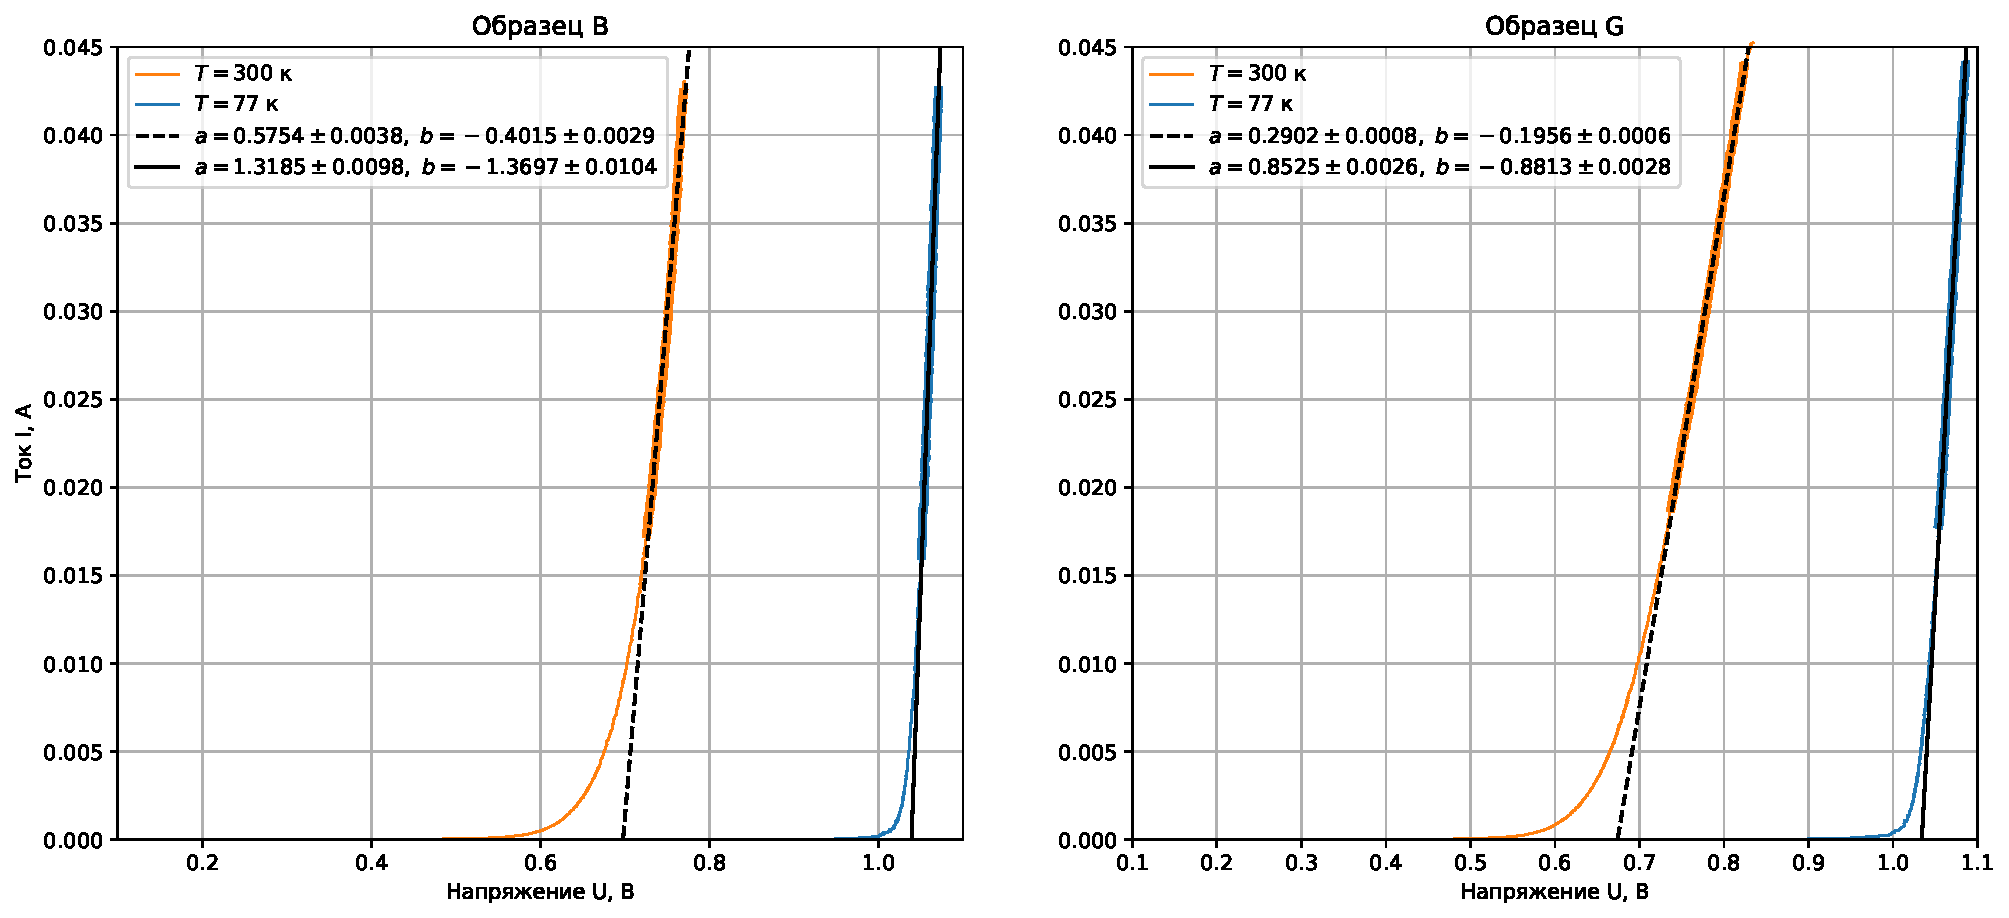
\includegraphics[width=\textwidth]{../figures/vi.pdf}
	\caption{Семейства вольт-амперных характеристик при различных температурах для образцов двух типов.}
		\label{fig:vi}
	\end{figure}
	Из линейной аппроксимации ВАХ мы находим некоторую прямую $I(U) = a U + b$, отсюда получаем для сопротивления толщи полупроводника $R_s = 1/a$ и $\Delta R_s = \Delta a/ a^2$, а для контактной разности потенциалов $\varphi_k = - b/a$ (определяется как точка пересечения с осью абсцисс) и $\Delta \varphi_k = (a \Delta b + b \Delta a )/a^2$. Результаты расчётов представлены на таблице \ref{tab:1}.

% Please add the following required packages to your document preamble:
% \usepackage{multirow}
\begin{table}[htbp]
\centering
\begin{tabular}{|c|c|c|c|c|c|}
\hline
Образец            & T, к & $R_s$, Ом & $\Delta R_s$, Ом & $\varphi_k$, В & $\Delta\varphi_k$, В \\ \hline
\multirow{2}{*}{B} & 300                     & 1.7379    & 0.0115           & 0.6978         & 0.0003               \\ \cline{2-6} 
                   & 77                      & 0.7585    & 0.0057           & 1.0389         & 0.0002               \\ \hline
\multirow{2}{*}{G} & 300                     & 3.4454    & 0.0090           & 0.6740         & 0.0003               \\ \cline{2-6} 
                   & 77                      & 1.1730    & 0.0036           & 1.0338         & 0.0001               \\ \hline
\end{tabular}
\caption{Результаты расчёта сопротивления толщи полупроводника и запирающего напряжения.}
\label{tab:1}
\end{table}

\Section{ОБРАБОТКА ВОЛЬТ-ФАРАДНЫХ ХАРАКТЕРИСТИК}

Требовалось обработать результаты измерений вольт-фарадных характеристик диода при обратном смещении $C(U)$, построив зависимости $(S/C)^2$ от $U$, где $S$ --- площадь р-n перехода (круг диаметром $0.8$ мм). Определить величины приведённой концентрации примесей в р-n переходе $N^*$, полной толщины истощённого слоя р-n перехода $l$ и контактной разности потенциала $\varphi_k$.

\Subsection{МАСШТАБИРОВАНИЕ ЕДИНИЦ ИЗМЕРЕНИЯ ЁМКОСТИ}

В эксперименте ёмкость мерилась в неких условных единицах. Чтобы понять, какие это единицы, была подключена ёмкость 39 пФ. Кроме того, такое измерение позволило определить настоящий нуль измеряемой ёмкости.

Чтобы получить из ёмкости $C_\text{wrong}$ в непонятных единицах ёмкость $C_\text{pF}$ в пФ надо:
$$
C_\text{pF} = \frac{(C_\text{wrong} - C_0)}{A}\,\times\,39\,\mathrm{пФ},
$$
где величина $C_0$ соответствует ложному нулю в условных единицах, а $A$ определяется как величина ёмкости 39 пФ, измеренная в условных единицах (с уже вычтенной $C_0$).

\Subsection{ЗАВИСИМОСТЬ $\mathbf{(S/C)^2}$ ОТ $\mathbf{U}$}

Теория даёт зависимость 
\begin{equation}
	C = S \sqrt{\frac{\varepsilon \varepsilon_0 q}{2} \frac{N^*}{\varphi_k - U}},
\end{equation}
откуда находим
\begin{equation}
	\qty(\frac{S}{C})^2 = \frac{2}{\varepsilon \varepsilon_0 q N^*} (\varphi_k - U).
\end{equation}
Такая линейная зависимость справедлива лишь при малых напряжениях, поэтому линейной регрессии подвергались лишь первые 100 точек каждого из наборов данных. То есть находились параметры $a$ и $b$ для линейной функции $aU+b$. Через эти параметры регрессии искомые физические параметры выражаются следующим образом:
\begin{equation}
 	\begin{split}
 		N^* = \dfrac{2}{\epsilon\epsilon_0 e a},\quad \Delta N^* = \dfrac{2\Delta a}{\epsilon\epsilon_0 e a^2};\\
 		\varphi_k = \frac{b}{a},\quad \Delta \varphi_k = \dfrac{b \Delta a + a \Delta b}{a^2};\\
 		l_0 = \epsilon\epsilon_0\sqrt{b},\quad \Delta l_0 = \dfrac{b \epsilon\epsilon_0}{2 \sqrt{b}}.
 	\end{split}
 \end{equation}
 Результаты расчётов приведены в таблице \ref{tab:2}.

 % Please add the following required packages to your document preamble:
% \usepackage{multirow}
\begin{table}[htbp]
\begin{tabular}{|c|c|c|c|c|c|c|}
\hline
Образец            & T, ${}^\circ\mathrm{C}$ & $N^*$, $\times10^{21}$ м${}^{-3}$ & $\varphi_k$, В & $\Delta\varphi_k$, В & $l_0$, мкм & $\Delta l_0$, мкм \\ \hline
\multirow{2}{*}{B} & 300                     & 1.40                              & 0.581          & 0.005                & 0.741      & 0.003             \\ \cline{2-7} 
                   & 77                      & 1.38                              & 1.200          & 0.007                & 1.07       & 0.002             \\ \hline
\multirow{2}{*}{G} & 300                     & 1.41                              & 0.724          & 0.006                & 0.825      & 0.003             \\ \cline{2-7} 
                   & 77                      & 1.42                              & 1.150          & 0.003                & 1.03       & 0.001             \\ \hline
\end{tabular}
\caption{Результаты расчёта приведённой концентрации примесей в р-n переходе $N^*$, полной толщины истощённого слоя р-n перехода $l$ и контактной разности потенциала $\varphi_k$.}
\label{tab:2}
\end{table}

\end{document}